%!TEX root =../mapp-challenge-18-game-book.tex
% ^ leave for LaTeXTools build functionality

\phChapterWorksheet{Go Get 'Em!}{Main Puzzle 1}

While traveling down Road \(4.139\pi\),
you cross paths with a wizened \mappMobimon{} Trainer. After finally
completing his
\textbf{non-skippable seven-hour tutorial} on how to catch \mappMobimon{},
you try to slip away without him noticing. Alas, before you can make your
excuses, he begins to tell you how \mappMobimon{} battles were fought
\textbf{back in his day}.

Before \mappMobimon{} battles were limited to one-on-one matches,
two trainers would send all their \mappMobimon{} into battle at once. Trainers
would often practice battling by placing \textbf{black and white stones}
on the \textbf{intersections of lines on a grid}, representing the positions
of each trainer's \mappMobimon{}. The old man,
not bothering to hide his frustration that you aren't showing any
interest in this bit of history, insists on showing you the following examples.

\begin{center}
  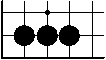
\includegraphics{gogetem/assets/explanation1-crop}
  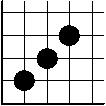
\includegraphics{gogetem/assets/explanation2-crop}
\end{center}

The senile old coot explains that the left figure is an example of a single
\textbf{group} because the stones are directly adjacent horizontally
or vertically on the board, but the right figure represents
three separate groups of stones.

To defeat a group of stones, it seems that you are required to
\textbf{completely surround the group with your own stones}. As illustrated
in the old man's next examples, the x's mark where white stones would need to be
played to capture all the black stones.

\begin{center}
  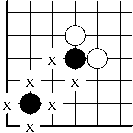
\includegraphics{gogetem/assets/explanation3-crop}
  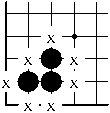
\includegraphics{gogetem/assets/explanation4-crop}
\end{center}

Normally you \textbf{can't play a stone if it doesn't have some empty space next
to it.} The one exception is that you can play a stone if that play
\textbf{creates empty space by capturing your opponent's stones.} 

You haven't really been listening, but then the old man mentions that he
might be able to tell you where to \textbf{find some interesting Plant-type
\mappMobimon{}} if you can solve a related \textbf{puzzle}.
In each of the provided \textbf{Old-School \mappMobimon{} Battle Grids},
there is exactly one position where a stone
could be played (white or black) to defeat a group of opposite-colored stones.
Solve his puzzle by taking the boundary letters
that match the color and position of the correct stone for each grid
(and then get out of there before the old man can start another long-winded
conversation!).

\phWorksheet{Old-School \mappMobimon{} Battle Grids}

% To make the cropped boards,
% Easy way (macOS/*nix/cygwin): open a terminal, cd into assets and type "make"
% Hard way: Build all of boards#.tex, then in a terminal run pdfcrop on all of
%           the resulting boards#.pdf files.
\begin{center}
  \contournumber{64}
  \resizebox{6in}{!}{
  \begin{tikzpicture}
    \node[anchor=south west,inner sep=0] (image) at
    (0,0){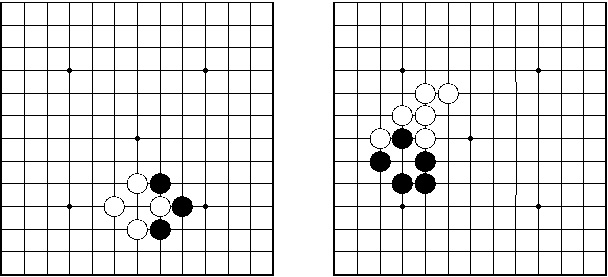
\includegraphics[scale=1.5]{gogetem/assets/boards1-crop}};
    % left board coordinate system
    \foreach \x in {0,...,12}
    \node at (\x * 0.58, 7.3){\contour{black}{\AlphAlph{\x + 14}}};
    \foreach \x in {0,...,12}
    \node at (-0.25, \x * 0.58){\contour{black}{\textcolor{white}{\AlphAlph{13 -
          \x}}}};
    % right board coordinate system
  \foreach \x in {0,...,12} \node at (8.5 + \x * 0.58,
  7.3){\contour{black}{\AlphAlph{\x + 14}}}; \foreach \x in {0,...,12} \node at
  (8.2, \x * 0.58){\contour{black}{\textcolor{white}{\AlphAlph{13 - \x}}}};
  \end{tikzpicture}
  }

  \vfill

  \resizebox{6in}{!}{
  \begin{tikzpicture}
    \node[anchor=south west,inner sep=0] (image) at
    (0,0){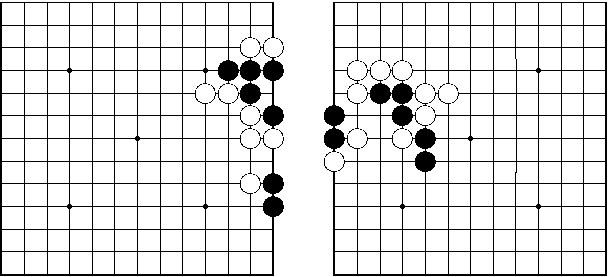
\includegraphics[scale=1.5]{gogetem/assets/boards2-crop}};
    % left board coordinate system
    \foreach \x in {0,...,12}
    \node at (\x * 0.58, 7.3){\contour{black}{\AlphAlph{\x + 14}}};
    \foreach \x in {0,...,12}
    \node at (-0.25, \x * 0.58){\contour{black}{\textcolor{white}{\AlphAlph{13 -
          \x}}}};
    % right board coordinate system
    \foreach \x in {0,...,12}
    \node at (8.5 + \x * 0.58, 7.3){\contour{black}{\AlphAlph{\x + 14}}};
    \foreach \x in {0,...,12}
    \node at (8, \x * 0.58){\contour{black}{\textcolor{white}{\AlphAlph{13 - \x}}}};
  \end{tikzpicture}
  }

  \vfill
  \newpage

  \resizebox{6in}{!}{
  \begin{tikzpicture}
    \node[anchor=south west,inner sep=0] (image) at
    (0,0){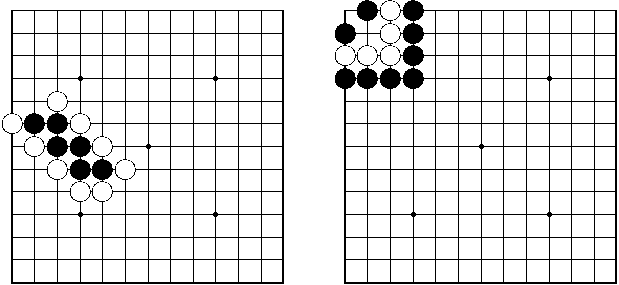
\includegraphics[scale=1.5]{gogetem/assets/boards3-crop}};
    % left board coordinate system
    \foreach \x in {0,...,12}
    \node at (0.35 + \x * 0.58, 7.6){\contour{black}{\AlphAlph{\x + 14}}};
    \foreach \x in {0,...,12}
    \node at (-0.25, \x * 0.58){\contour{black}{\textcolor{white}{\AlphAlph{13 -
          \x}}}};
    % right board coordinate system
    \foreach \x in {0,...,12}
    \node at (8.7 + \x * 0.58, 7.5){\contour{black}{\AlphAlph{\x + 14}}};
    \foreach \x in {0,...,12}
    \node at (8.2, \x * 0.58){\contour{black}{\textcolor{white}{\AlphAlph{13 - \x}}}};
  \end{tikzpicture}
  }

  \vfill

  \resizebox{6in}{!}{
  \begin{tikzpicture}
    \node[anchor=south west,inner sep=0] (image) at
    (0,0){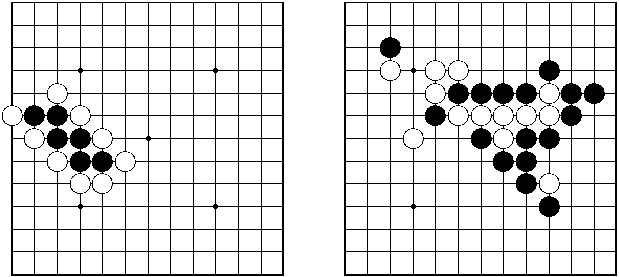
\includegraphics[scale=1.5]{gogetem/assets/boards4-crop}};
    % left board coordinate system
    \foreach \x in {0,...,12}
    \node at (0.3 + \x * 0.58, 7.5){\contour{black}{\AlphAlph{\x + 14}}};
    \foreach \x in {0,...,12}
    \node at (-0.25, \x * 0.58){\contour{black}{\textcolor{white}{\AlphAlph{13 -
          \x}}}};
    % right board coordinate system
    \foreach \x in {0,...,12}
    \node at (8.7 + \x * 0.58, 7.3){\contour{black}{\AlphAlph{\x + 14}}};
    \foreach \x in {0,...,12}
    \node at (8.2, \x * 0.58){\contour{black}{\textcolor{white}{\AlphAlph{13 - \x}}}};
  \end{tikzpicture}
  }

  \vfill

  \resizebox{3in}{!}{
  \begin{tikzpicture}
    \node[anchor=south west,inner sep=0] (image) at
    (0,0){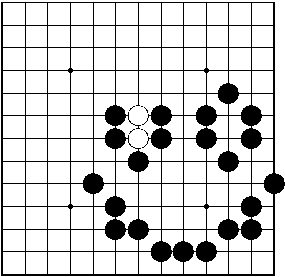
\includegraphics[scale=1.5]{gogetem/assets/boards5-crop}};
    % left board coordinate system
    \foreach \x in {0,...,12}
    \node at (\x * 0.58, 7.3){\contour{black}{\AlphAlph{\x + 14}}};
    \foreach \x in {0,...,12}
    \node at (-0.25, \x * 0.58){\contour{black}{\textcolor{white}{\AlphAlph{13 -
          \x}}}};
  \end{tikzpicture}
  }

\end{center}

% Include below for aucTeX integration
%%% Local Variables:
%%% mode: latex
%%% TeX-master: "../mapp-challenge-18-game-book"
%%% End:
